\chapter{Desarrollo}

\section{ Compare los valores teóricos y prácticos de la tabla de respuestas y encuentre los errores porcentuales}

En la tabla resumen \ref{tab:valores-salida-rect} se puede apreciar los resultados medidos para un $V_{RMS}$ de entrada para cada línea de \textbf{12V} en la implementación a nivel de simulación en comparación con los valores teóricos obtenidos a partir de las relaciones definidas para el rectificador trifásico controlado a media onda.


\begin{table}[h]
	\centering
	\begin{tabular}{|l|ccc|ccc|ccc|}
		\hline
		\multicolumn{1}{|c|}{\multirow{2}{*}{\textbf{Valores}}} & \multicolumn{3}{c|}{\textbf{Para $\alpha$ = 110º}}                                                      & \multicolumn{3}{c|}{\textbf{Para $\alpha$ = 80º}}                                                       & \multicolumn{3}{c|}{\textbf{Para $\alpha$ = 50º}}                                                       \\ \cline{2-10} 
		\multicolumn{1}{|c|}{}                                  & \multicolumn{1}{c|}{\textbf{Teórico}} & \multicolumn{1}{c|}{\textbf{Práctico}} & \textbf{E (\%)} & \multicolumn{1}{c|}{\textbf{Teórico}} & \multicolumn{1}{c|}{\textbf{Práctico}} & \textbf{E (\%)} & \multicolumn{1}{c|}{\textbf{Teórico}} & \multicolumn{1}{c|}{\textbf{Práctico}} & \textbf{E (\%)} \\ \hline
		\textbf{Pot}                                       & \multicolumn{1}{c|}{9.51}             & \multicolumn{1}{c|}{9.50}              & 0.11                & \multicolumn{1}{c|}{5.33}             & \multicolumn{1}{c|}{5.35}              & 0.38                & \multicolumn{1}{c|}{1.9}              & \multicolumn{1}{c|}{1.9}               & 0                   \\ \hline
		\textbf{Vdc}                                         & \multicolumn{1}{c|}{11.48}            & \multicolumn{1}{c|}{11.40}             & 0.70                & \multicolumn{1}{c|}{7.87}             & \multicolumn{1}{c|}{7.68}              & 2.41                & \multicolumn{1}{c|}{3.75}             & \multicolumn{1}{c|}{3.74}              & 0.27                \\ \hline
		\textbf{Vrms}                                           & \multicolumn{1}{c|}{0.634}            & \multicolumn{1}{c|}{0.633}             & 0.16                & \multicolumn{1}{c|}{0.355}            & \multicolumn{1}{c|}{0.357}             & 0.56                & \multicolumn{1}{c|}{0.127}            & \multicolumn{1}{c|}{0.127}             & 0                   \\ \hline
		\textbf{Idc}                                         & \multicolumn{1}{c|}{0.765}            & \multicolumn{1}{c|}{0.760}             & 0.65                & \multicolumn{1}{c|}{0.525}            & \multicolumn{1}{c|}{0.512}             & 2.48                & \multicolumn{1}{c|}{0.250}            & \multicolumn{1}{c|}{0.249}             & 0.40                \\ \hline
		\textbf{Irms}                                           & \multicolumn{1}{c|}{8.78}             & \multicolumn{1}{c|}{8.66}              & 1.37                & \multicolumn{1}{c|}{4.14}             & \multicolumn{1}{c|}{3.93}              & 4.84                & \multicolumn{1}{c|}{0.938}            & \multicolumn{1}{c|}{0.932}             & 0.64                \\ \hline
	\end{tabular}
	\caption{Valores eléctricos de salida - Rectificador controlado trifásico media onda}
	\label{tab:valores-salida-rect}
\end{table}


De los valores obtenidos se puede apreciar una gran fidelidad o cercanía entre los valores experimentales y los teóricos con errores porcentuales cercanos a cero destacando la importancia de un correcto control en los tiempos de activación de cada SCR (tiristor) en conjunto al detector de cruce por cero que permite identificar el inicio de un nuevo ciclo facilitando el control de los retardos e interrupciones programadas en el microcontrolador.

\begin{figure}[h]
	\centering
	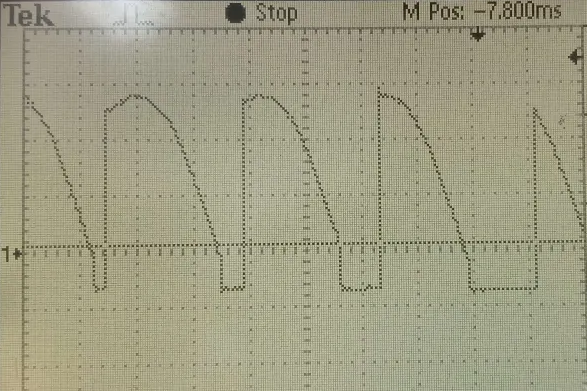
\includegraphics[width=0.7\linewidth]{media/salida-rect-controlado}
	\caption{Forma de onda de salida para el rectificador trifásico controlador a media onda}
	\label{fig:salida-rect-controlado}
\end{figure}

Para validar los datos emulados en la implementación se considero un voltaje de alimentación de 47v y un angulo de disparo ($\alpha = 50º$) y cuya salida salida se muestra en la figura \ref{fig:salida-rect-controlado} y la cual presenta algunas distorsiones en la forma de onda esto debido a pequeñas variaciones en los desfases entre líneas y los tiempos de retardo para la activación de los SCR desde Arduino.










